\chapter{Evaluation}
\label{chap:evaluation}

\noteinfo[inline]{Remember to describe that we could not get the network stack
down on the FPGA}
\section{Setup}
In the initial stages of testing, the components had simulation processes between
block. This made it possible to implement different blocks of the system
independent of each other.\\
These tests where changing a lot, because the initial design where not
reached yet.
When the modules where done, they where wired together and a simulator
where created to handle all input and output of the system.

\subsection{Graph file simulator}
\begin{figure*}[t!]
    \centering
    \begin{subfigure}[b]{0.16\textwidth}
        \centering
        \includegraphics[scale=0.45]{evaluation/dot_files/datain.eps}
        \caption{Data In}
        \label{fig:packet_graph_datain}
    \end{subfigure}%
    \begin{subfigure}[b]{0.16\textwidth}
        \centering
        
\includegraphics[scale=0.45]{evaluation/dot_files/send.eps}
        \caption{Send}
        \label{fig:packet_graph_send}
    \end{subfigure}%
    \begin{subfigure}[b]{0.16\textwidth}
        \centering
        \includegraphics[scale=0.45]{evaluation/dot_files/command.eps}
        \caption{Command}
        \label{fig:packet_graph_command}
    \end{subfigure}%
    \begin{subfigure}[b]{0.16\textwidth}
        \centering
        \includegraphics[scale=0.45]{evaluation/dot_files/dataout.eps}
        \caption{Data Out}
        \label{fig:packet_graph_dataout}
    \end{subfigure}%
    \begin{subfigure}[b]{0.16\textwidth}
        \centering
        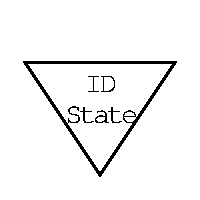
\includegraphics[scale=0.45]{evaluation/dot_files/receive.eps}
        \caption{Receive}
        \label{fig:packet_graph_receive}
    \end{subfigure}%
    \begin{subfigure}[b]{0.16\textwidth}
        \centering
        \includegraphics[scale=0.45]{evaluation/dot_files/wait.eps}
        \caption{Wait}
        \label{fig:packet_graph_wait}
    \end{subfigure}%
    \caption{The different node types in the simulation graph}
    \label{fig:packet_dot_files}
\end{figure*}%
The graph simulator is an abstract structure for easily composition and
illustrations of simulations in the system. The system can be boiled down
to inputs(sources) and output(sinks). The code is deterministic, since the same
combination of input and output signals would result in the exact same internal
state of the system. This means that a simulation of the system as a whole would
require knowing what to write/read at every source/sink, and doing it at the
right time. However, we do not need the timing on a clock to clock basis, since
the external network does not care when the system sends out a packet, only
if the packet is structured correctly. The user however may need information
regarding the latency of the system. The latency is based on the
specific system state, and is described in
\autoref{subsec:latency}.\\
With these assumptions it is possible to illustrate the timeline of the packets
with a graph, where a vertex does action on a clock to clock basis(etc. sending a
packet into the system.), and each edge describes what node to proceed to.
Each vertex have a state. When the \texttt{Done} state is reached
the next vertex is set to the \texttt{Ready} state, but only if
they are connected via an edge. If a vertex contains multiple ingoing edges, each
vertex with outgoing edges to that vertex needs to be \texttt{Done}.\\
{\renewcommand{\arraystretch}{1.3}
\begin{table}[htpb]
    \begin{center}
        \begin{tabular}{lcl}
            State & Color&Description\\ \hline \hline
            \texttt{Waiting}& \statecolorbox{graph_waiting} &
            \makecell{Vertex is not in use.}\\ \hline

            \texttt{Ready}& \statecolorbox{graph_isready} &
            \makecell{Vertex Is ready\\ for activation.}\\ \hline

            \texttt{Active}& \statecolorbox{graph_active} &
            \makecell{Vertex is active.\\ Simulator is\\ gathering data.}\\ \hline

            \texttt{Inactive}& \statecolorbox{graph_inactive} &
            \makecell{Vertex is inactive.\\Simulator is not\\ gathering data.}\\ \hline

            \texttt{Done}& \statecolorbox{graph_done} &
            \makecell{Vertex is done\\ and validated.}
        \end{tabular}
    \end{center}
    \caption{The different states of the nodes, and their respective colors} \label{tab:graph_node_states}
  \end{table}
}\\
Each vertex have their own type, defining what input source or output sink to
use. The graph file simulator consists of multiple input sources and output sinks
as seen in \autoref{fig:packet_dot_files}.\\
There are three inputs, giving data to the system:
Data in(\subref{fig:packet_graph_datain}),
Send(\subref{fig:packet_graph_send}) and
Command(\subref{fig:packet_graph_command}).
There are two sinks, getting data from the system
Data out(\subref{fig:packet_graph_dataout}) and
Receive(\subref{fig:packet_graph_receive}).
The node type Wait(\subref{fig:packet_graph_wait}) is special, since
it does not use a input or a sink. It simply counts down each clock, until it's
counter reaches zero.\\
Since there only exist one of each input source and output sink (except Wait),
the simulator can only work on one vertex of each type at a time.
In graphs where there are multiple ready vertexes of same type, the vertex with
the lowest ID are focused on first. When a vertex is focused, it is set as
\texttt{Active}.\\
When the vertex is finished, it is set to \texttt{Done}.
An example of a graph can be seen in
\autoref{fig:graph_simulation_running_examples}.


\begin{figure*}[htpb]
    \centering
    \begin{subfigure}[b]{0.5\textwidth}
        \centering
        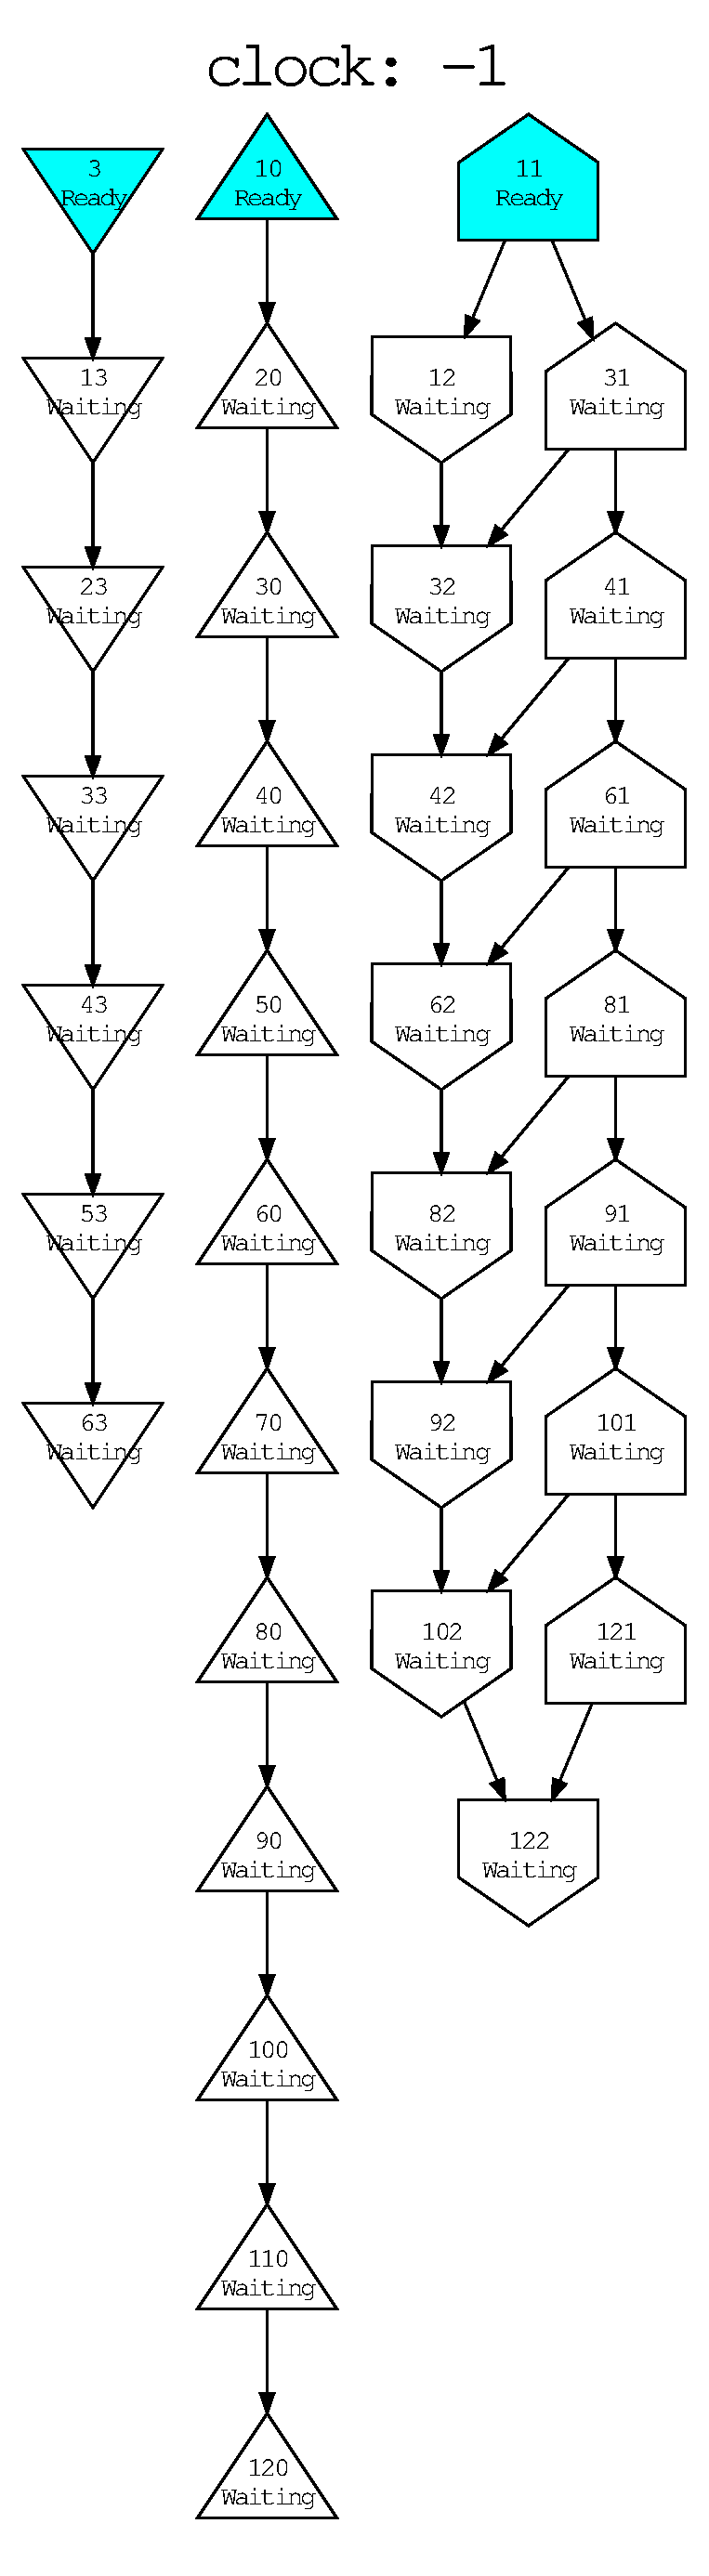
\includegraphics[scale=0.45]{evaluation/dot_files/example_graph_initial.eps}
        \caption{The initial state of a simulation}
        \label{fig:example_packet_graph_initial}
    \end{subfigure}%
    \begin{subfigure}[b]{0.50\textwidth}
        \centering
        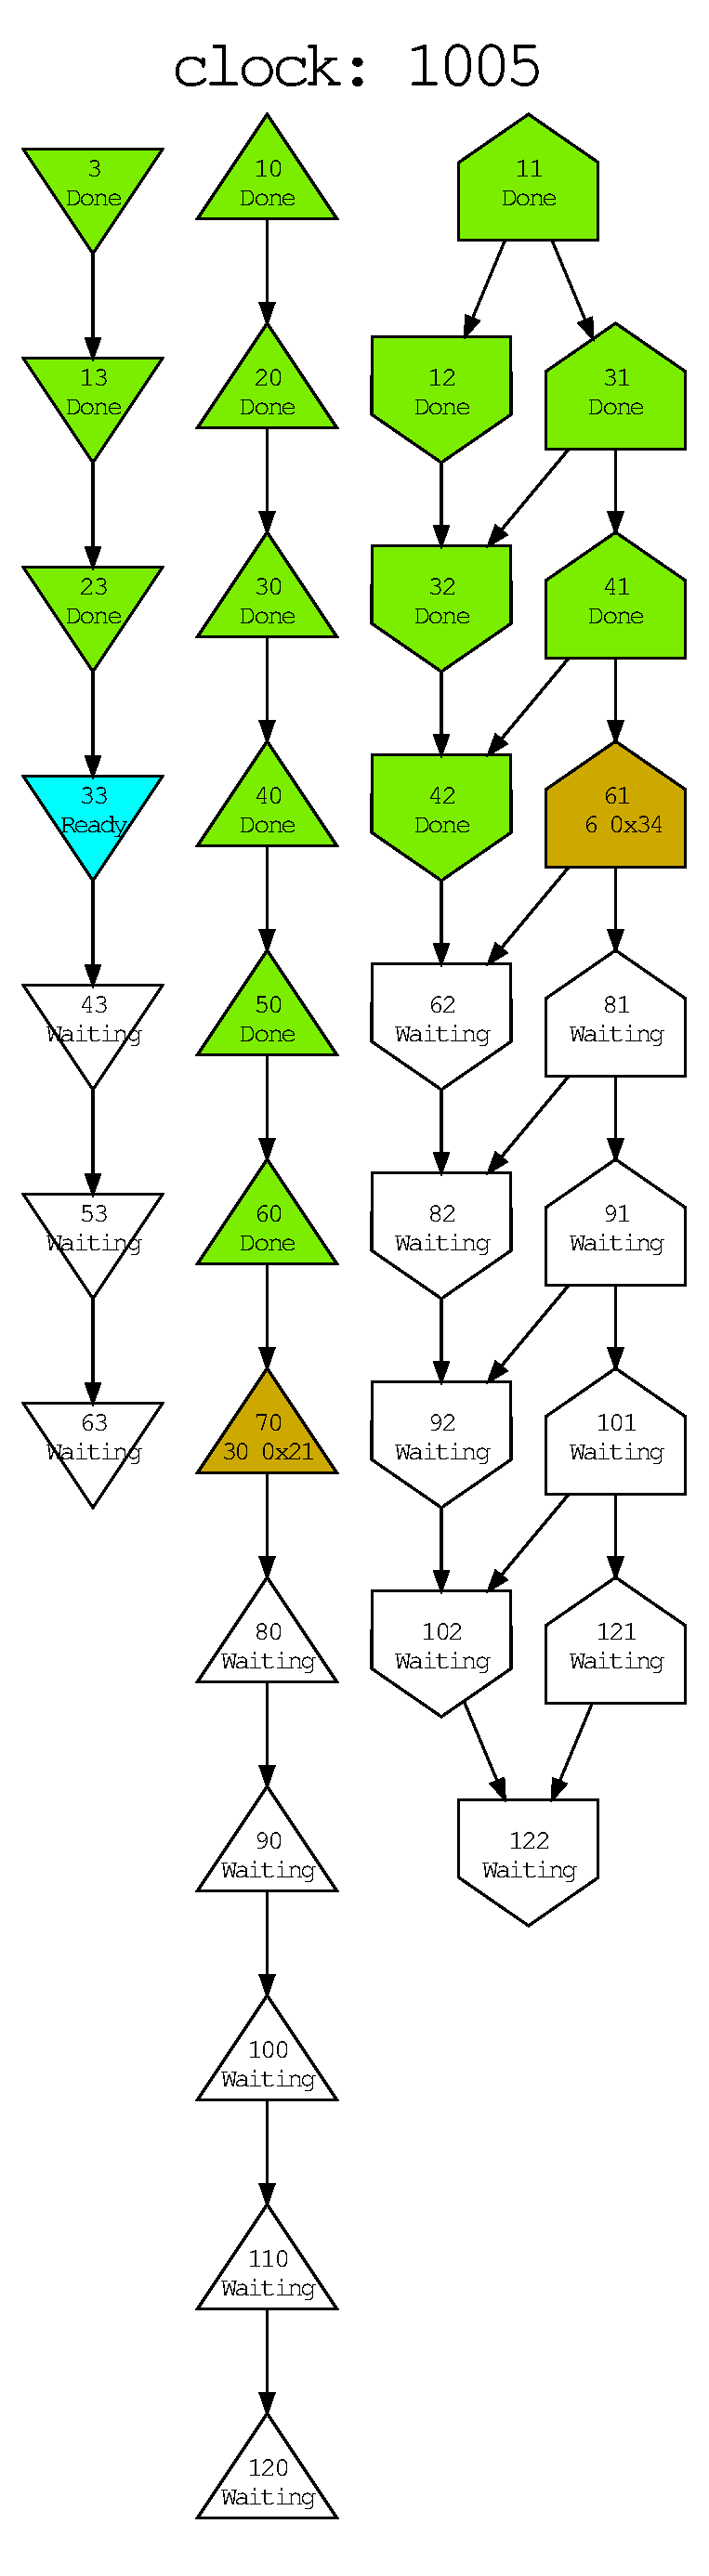
\includegraphics[scale=0.45]{evaluation/dot_files/example_graph_running.eps}
        \caption{The state after 1005 clocks}
        \label{fig:example_packet_graph_running}
 	\end{subfigure}%
    \caption{A Illustration of the graph states before running and 1005 clocks
    inside the simulation}
    \label{fig:graph_simulation_running_examples}
\end{figure*}



\section{Test}
\subsection{Latency}\label{subsec:latency}

\section{Verification}

